\subsection{Grobkonzept 4} \label{subsec:grobkonzept3}
\begin{table}[H]
\small
\begin{tabular}{>{\HY\RaggedRight}p{3cm} >{\HY\RaggedRight}p{3.6cm} >{\HY\RaggedRight}p{6.9cm} r}
\hline
\textbf{Bestandteil}&\textbf{Typ}&\textbf{Funktion}&\textbf{Anz.}\\
\hline

\rowcolor{hellgrau}
\multicolumn{4}{l}{\textbf{Stromerzeugung}}\T\\
Rohrkette&&Umwandlung potenzielle Energie zu Rotation&6\\
Zahnrad&&Umdehungszahl für Generator anpassen&6\\
Generator&AC&Umwandlung in elektrische Energie&6\\
Gleichrichter&AC/DC Wandler&Wechselstrom zu Gleichstrom&6\\
DC/DC Konverter&&Regelt die Spannung für den DC Bus&6\\
Wechselrichter&&Umwandlung DC in AC (230V)&1\B\\

\rowcolor{hellgrau}
\multicolumn{4}{l}{\textbf{Kontrollsystem}}\T\\
PC&&Anlagesteuerung&1\\
SPS&Beckhof&Analoge und Digitale Ein- und Ausgänge&1\B\\

\rowcolor{hellgrau}
\multicolumn{4}{l}{\textbf{Abwassertechnik}}\T\\
Ventile&Absperrklappe&Umleitung in Fallleitung für Wartungsarbeiten am Wasserlift&74\\
Fallleitung&&Für Wartungsarbeiten&1\B\\

\hline
\end{tabular}
\caption{Bestandteilliste Grobkonzept 4}\label{tab:BLGrobkonzept4}
\end{table}
Im Grobkonzept 4 wird die potenzielle Energie des Abwassers mit einem Wasserlift ausgenutzt. Der Lift besteht aus einer Umlaufenden Kette, an der runde, tellerförmige Schaufeln befestigt sind. Die Kette bewegt sich  durch zwei parallele, vertikal verlegte Rohre, im einen nach oben und im anderen nach unten. Am oberen und unteren Ende wird die Kette mit einem Rad in das andere Rohr umgelenkt. Das Abwasser fliesst aus dem jeweiligen Stockwerk in eine der Schaufeln und treibt den Lift durch sein Gewicht an. Das Abwasser wandert im Lift nach unten und wird am tiefsten Punkt entleert. Die Drehbewegung, welche die Rohrkette dabei erzeugt, ist eher langsam. Daher muss die Drehzahl mit einem Getriebe erhöht werden, damit die Mindestdrehzahl des Generators erreicht wird. Während Wartungsarbeiten wird das Abwasser mittels Ventilen in eine Fallleitung umgeleitet. Damit der Strom der Turbinen zusammengeführt werden kann, muss der Wechselstrom zuerst in Gleichstrom umgewandelt werden. Dieser wird auf einen DC-DC Konverter gelegt, damit kein Strom zurück in den Generator fliessen kann. Anschliessend wird der Gleichstrom mit einem Wechselrichter auf Netz-Spannung umgewandelt. Ein Kontrollsystem steuert die Anlage, überwacht die Energiegewinnung und schreitet bei Störungen ein. Die 5 oberen Lifte haben eine Länge von \(66.08m\), der unterste Lift \(80.24m\). Für Wartungsarbeiten existiert eine zusätzliche Leitung, die mittels Bypass angesteuert wird.
\newpage
\begin{wrapfigure}{r}{0.5\textwidth}
  \begin{center}
    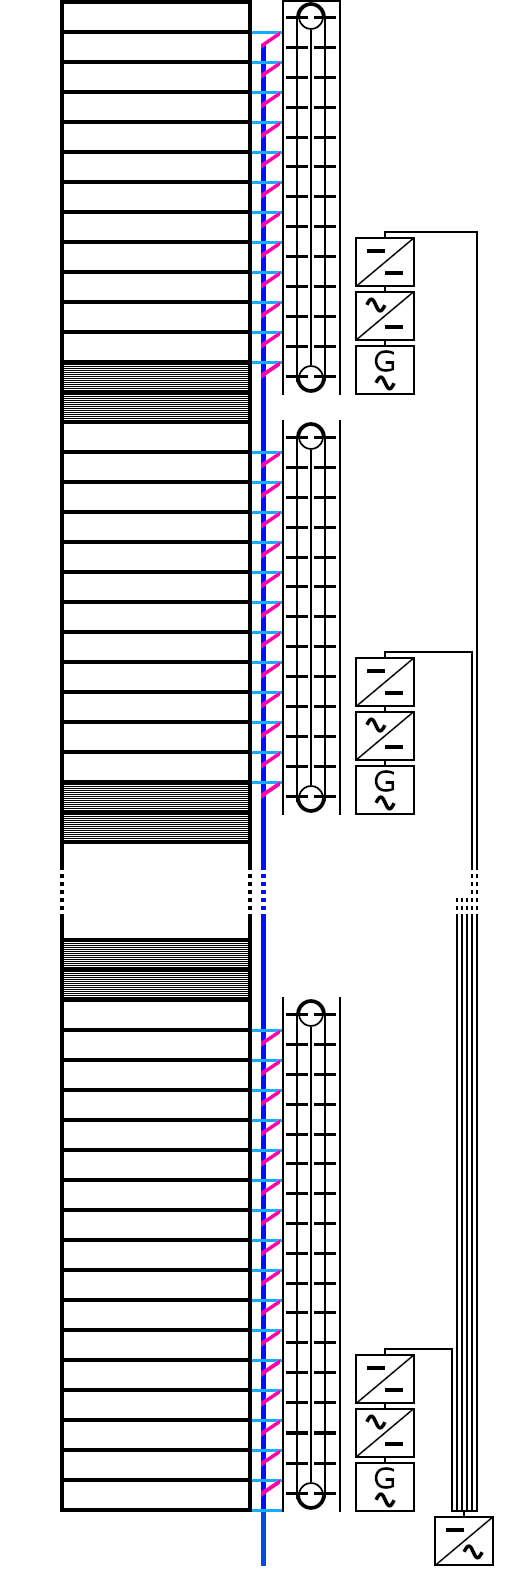
\includegraphics[width=0.48\textwidth]{grobkonzept4}
  \end{center}
  \caption{Grobkonzept 4}
\end{wrapfigure}


\textbf{Vorteile:}							\newline
+ 	platzsparend								\newline
\newline
\textbf{Nachteile:}\newline
-	viele Ventile								\newline
-	Lufwiderstand							\newline
\WFclear			
\newpage